% -*- latex -*-
%%%%%%%%%%%%%%%%%%%%%%%%%%%%%%%%%%%%%%%%%%%%%%%%%%%%%%%%%%%%%%%%
%%%%%%%%%%%%%%%%%%%%%%%%%%%%%%%%%%%%%%%%%%%%%%%%%%%%%%%%%%%%%%%%
%%%%
%%%% This text file is part of the source of 
%%%% `Parallel Programming in MPI and OpenMP'
%%%% by Victor Eijkhout, copyright 2012-2022
%%%%
%%%% mpi-running.tex : about running MPI programs
%%%%
%%%%%%%%%%%%%%%%%%%%%%%%%%%%%%%%%%%%%%%%%%%%%%%%%%%%%%%%%%%%%%%%
%%%%%%%%%%%%%%%%%%%%%%%%%%%%%%%%%%%%%%%%%%%%%%%%%%%%%%%%%%%%%%%%

\Level 0 {Starting and running MPI processes}
\label{sec:mpi-start}

The \ac{SPMD} model may be initially confusing. Even though there is
only a single source, compiled into a single executable,
the parallel run comprises a number of independently started MPI
processes (see section~\ref{sec:mpiexec} for the mechanism).

The following exercises are designed to give you an intuition for this
one-source-many-processes setup. In the first exercise you will see
that the mechanism for starting MPI programs starts up independent
copies. There is nothing in the source that says `and now you become parallel'.

\begin{figure}[ht]
  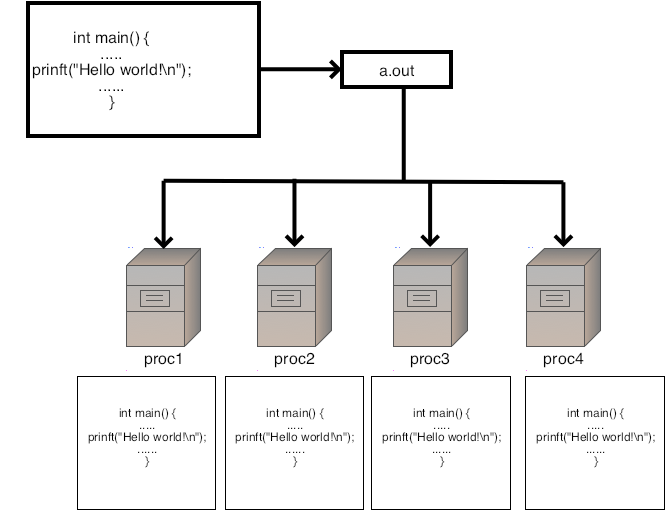
\includegraphics[scale=.45]{hello-parallel}
  \caption{Running a hello world program in parallel}
  \label{fig:hello-parallel}
\end{figure}

The following exercise demonstrates this point.

%pyinput ex-hello.txt

\begin{exercise}
  \label{ex:hello1}
  Write a `hello world' program, without any MPI in it,
  and run it in parallel with \indextermtt{mpiexec} or your local equivalent. 
  Explain the output.

\begin{tacc}
    (On TACC machines such as stampede, use \indextermtt{ibrun}, no
    processor count.)
\end{tacc}

  \skeleton{hello}
\end{exercise}

This exercise is illustrated in figure~\ref{fig:hello-parallel}.

\Level 1 {Headers}

If you use MPI commands in a program file, be sure to include
the proper header file, \indextermtt{mpi.h} or \indextermtt{mpif.h}.
\begin{verbatim}
#include "mpi.h" // for C
#include "mpif.h" ! for Fortran
\end{verbatim}
For \fstandard{90}, many MPI installations
also have an MPI module, so you can write
\begin{verbatim}
use mpi     ! pre 3.0
use mpi_f08 ! 3.0 standard
\end{verbatim}
The internals of these files can be different between MPI
installations, so you can not compile one file against one \n{mpi.h}
file and another file, even with the same compiler on the same machine,
against a different MPI.

\begin{pythonnote}{Import mpi module}
  It's easiest to
\begin{lstlisting}
from mpi4py import MPI
\end{lstlisting}
\end{pythonnote}

\begin{mplnote}{Header file}
  To compile MPL programs, add a line
\begin{lstlisting}
#include <mpl/mpl.hpp>
\end{lstlisting}
  to your file.
\end{mplnote}

\Level 1 {Initialization / finalization}
\label{sec:mpi-init}

Every (useful) MPI program has to start with \indextermbus{MPI}{initialization}
through a call to
\indexmpiref{MPI_Init}, and have
\indexmpiref{MPI_Finalize} to finish the use of MPI in your program.
The init call is different between the various languages.

In~C, you can pass \indextermtt{argc} and \indextermtt{argv}, the arguments
of a C language main program:
 \begin{lstlisting}
int main(int argc,char **argv) {
    ....
    return 0;
}
\end{lstlisting}
(It is allowed to pass \n{NULL} for these arguments.)

Fortran (before 2008) lacks this commandline argument handling,
so \indexmpishow{MPI_Init} lacks those arguments.

\begin{pythonnote}{Initialize/finalize}
  In many cases,  no initialize and finalize calls are needed:
  the statement
  \verbatimsnippet{pympiimport}
  performs the initialization.
  Likewise, the finalize happens at the end of the program.

  However, for special cases, there is an \lstinline{mpi4py.rc} object
  that can be set in between importing \lstinline{mpi4py} and
  importing \lstinline{mpi4py.MPI}:
\begin{lstlisting}
import mpi4py
mpi4py.rc.initialize = False
mpi4py.rc.finalize = False
from mpi4py import MPI
MPI.Init()
# stuff
MPI.Finalize()
\end{lstlisting}
\end{pythonnote}

\begin{mplnote}{Init, finalize}
  There is no initialization or finalize call.
  \begin{mplimpl}
    Initialization is done at the first \lstinline+mpl::environment+ method call,
    such as \lstinline+comm_world+.
  \end{mplimpl}

\end{mplnote}

This may look a bit like declaring `this is the parallel part of a
program', but that's not true: again, the whole code is executed
multiple times in parallel.

\begin{exercise}
  \label{ex:hello2}
  Add the commands \indexmpishow{MPI_Init} and \indexmpishow{MPI_Finalize}
  to your code. Put three different print statements in your code: one before the init,
  one between init and finalize, and one after the finalize. Again explain the output.

  Run your program on a large scale, using a batch job.
  Where does the output go?
  Experiment with
\begin{verbatim}
MY_MPIRUN_OPTIONS="-prepend-rank" ibrun yourprogram
\end{verbatim}
\end{exercise}

\begin{remark}
  For hybrid MPI-plus-threads programming there is also a call
  \indexmpishow{MPI_Init_thread}. For that, see
  section~\ref{sec:init-thread}.
\end{remark}

\Level 2 {Aborting an MPI run}

Apart from \indexmpishow{MPI_Finalize}, which signals a successful
conclusion of the MPI run, an abnormal end to a run can be forced by
\indexmpiref{MPI_Abort}.
%
This stop execution on all processes associated with the communicator,
but many implementations will terminate all processes. The \n{value} parameter
is returned to the environment.

\csnippetwithoutput{abortcode}{code/mpi/c}{return}

\Level 2 {Testing the initialized/finalized status}

The commandline arguments \n{argc} and \n{argv} are only guaranteed to
be passed to process zero, so the best way to pass commandline information
is by a broadcast (section~\ref{sec:bcast}).

There are a few commands, such as
\indexmpishow{MPI_Get_processor_name}, that are allowed before
\indexmpishow{MPI_Init}.

If MPI is used in a library, MPI can have already been initialized in a main program.
For this reason, one can test where \indexmpishow{MPI_Init} has been called with
%
\indexmpiref{MPI_Initialized}.

You can test whether \indexmpishow{MPI_Finalize} has been called with
%
\indexmpiref{MPI_Finalized}.

\Level 2 {Information about the run}

Once MPI has been initialized, the \indexmpishow{MPI_INFO_ENV} object
contains a number of key/value pairs describing run-specific
information; see section~\ref{sec:mpi-info-env}.

\Level 2 {Commandline arguments}

The \indexmpishow{MPI_Init} routines takes a reference to \indextermtt{argc}
and \indextermtt{argv} for the following reason: the \indexmpishow{MPI_Init} calls
filters out the arguments to \indexterm{mpirun} or \indextermtt{mpiexec},
thereby lowering the value of \n{argc} and elimitating some of the \n{argv}
arguments.

On the other hand, the commandline arguments that are meant for \indextermtt{mpiexec}
wind up in the \indexmpishow{MPI_INFO_ENV} object as a set of
key/value pairs; see section~\ref{sec:mpi-info}.

